\begin{name}
	{\tenchude}{\tendethi}{LỚP TOÁN THẦY PHÁT}{\thoigian}
\end{name}
	
\setcounter{ex}{0}\setcounter{bt}{0}
\Opensolutionfile{ans}[ans/ans-2-TT-21-TranPhu-VinhPhuc-L4-23]
\begin{ex}%[Thi Chuyên Đề Lần 4 lớp 12 - THPT Trần Phú - Vĩnh Phúc - 23]%[Phan Anh - EX6-2023]%[2D2Y1-2]
	Với $a$ là số thực dương tùy ý, $\sqrt[3]{a^2}$ bằng
	\choice
	{$a^{\tfrac{3}{2}}$}
	{$\dfrac{2a}{3}$}
	{\True $a^{\tfrac{2}{3}}$}
	{$\dfrac{3a}{2}$}
	\loigiai{Ta có $\sqrt[3]{a^2}=a^{\tfrac{2}{3}}$.}
\end{ex}
\begin{ex}%[Thi Chuyên Đề Lần 4 lớp 12 - THPT Trần Phú - Vĩnh Phúc - 23]%[Phan Anh - EX6-2023]%[2D2Y6-1]
	Tập nghiệm $S$ của bất phương trình $\left(\dfrac{1}{3}\right)^{x^2-4}\ge27$ chứa bao nhiêu số nguyên
	\choice
	{\True $3$}
	{$1$}
	{$2$}
	{Vô số}
	\loigiai{Ta có $\left(\dfrac{1}{3}\right)^{x^2-4}\ge27\Leftrightarrow3^{4-x^2}\ge3^3\Leftrightarrow4-x^2\ge3\Leftrightarrow x^2-1\le0\Leftrightarrow-1\le x\le1$.\\
		Suy ra các nghiệm nguyên của bất phương trình là $\{-1;0;1\}$.}
\end{ex}
\begin{ex}%[Thi Chuyên Đề Lần 4 lớp 12 - THPT Trần Phú - Vĩnh Phúc - 23]%[Phan Anh - EX6-2023]%[1D3Y3-3]
	Cho cấp số cộng $\left(u_n\right)$ có $u_1=11$ và công sai $d=4$. Số hạng thứ ba bằng
	\choice
	{$44$}
	{$176$}
	{\True $19$}
	{$15$}
	\loigiai{Ta có $u_3=u_1+2d=11+2\cdot4=19$.}
\end{ex}
\begin{ex}%[Thi Chuyên Đề Lần 4 lớp 12 - THPT Trần Phú - Vĩnh Phúc - 23]%[Phan Anh - EX6-2023]%[2D3Y1-1]
	Hàm số $F(x)=\dfrac{1}{3}x^3-2x^2+x-2021$ là một nguyên hàm của hàm số nào dưới đây?
	\choice
	{$f(x)=\dfrac{1}{9}x^4+\dfrac{2}{3}x^3-\dfrac{1}{2}x^2-2021x+C$}
	{$f(x)=\dfrac{1}{12}x^4-\dfrac{2}{3}x^3+\dfrac{1}{2}x^2-2021x+C$}
	{$f(x)=\dfrac{1}{9}x^4-\dfrac{2}{3}x^3+\dfrac{1}{2}x^2-2021x+C$}
	{\True $f(x)=x^2-4x+1$}
	\loigiai{Ta có $F'(x)=x^2-4x+1$ nên $F(x)$ là nguyên hàm của hàm số $f(x)=x^2-4x+1$}
\end{ex}
\begin{ex}%[Thi Chuyên Đề Lần 4 lớp 12 - THPT Trần Phú - Vĩnh Phúc - 23]%[Phan Anh - EX6-2023]%[2D1Y2-2]
	\immini{Cho hàm số $y=f(x)$ có đồ thị như hình vẽ. Số điểm cực trị của hàm số là
		\choice
		{$1$}
		{$0$}
		{$3$}
		{\True $2$}}
	{
		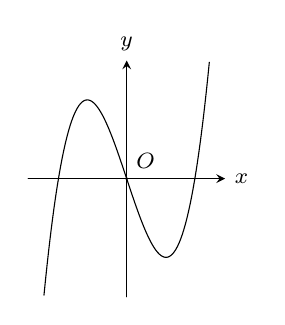
\begin{tikzpicture}[>=stealth,line join=round,line cap=round,font=\footnotesize,scale=0.5]
			\draw[->] (-2.5,0)--(2.5,0) node[right] {$x$};
			\draw[->] (0,-3)--(0,3) node[above] {$y$};
			\draw [smooth,domain=-2.1:2.1,samples=100]plot(\x,{(\x)^3-3*(\x)});
			\fill (0,0)node[above right]{\footnotesize{$O$}}circle(1.2pt);
	\end{tikzpicture}}
	\loigiai{Dựa vào đồ thị, ta thấy hàm số có hai điểm cực trị.}
\end{ex}
\begin{ex}%[Thi Chuyên Đề Lần 4 lớp 12 - THPT Trần Phú - Vĩnh Phúc - 23]%[Phan Anh - EX6-2023]%[2D1Y3-1]
	\immini{Cho hàm số $y=f(x)$ có đồ thị như hình vẽ. Giá trị lớn nhất và giá trị nhỏ nhất của hàm số đã cho trên $[-1;1]$ lần lượt là
		\choice
		{\True $-3$ và $-4$}
		{$1$ và $-4$}
		{$0$ và $-4$}
		{$1$ và $-1$}}
	{
		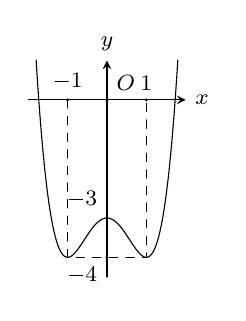
\begin{tikzpicture}[>=stealth,line join=round,line cap=round,font=\footnotesize,scale=0.5]
			\draw[->] (-2,0)--(2,0) node[right] {$x$};
			\draw[->] (0,-4.5)--(0,1) node[above] {$y$};
			\draw [smooth,domain=-1.8:1.8,samples=100]plot(\x,{(\x)^4-2*(\x)^2-3});
			\draw[dashed](-1,0)--(-1,-4)--(1,-4)--(1,0);
			\fill (0,0)node[above right]{\footnotesize{$O$}}circle(1.2pt) (1,0)node[above]{\footnotesize{$1$}}circle(1.2pt) (-1,0)node[above]{\footnotesize{$-1$}}circle(1.2pt) (0,-3)node[above left]{\footnotesize{$-3$}}circle(1.2pt)  (0,-4)node[below left]{\footnotesize{$-4$}}circle(1.2pt);
	\end{tikzpicture}}
	\loigiai{Dựa vào đồ thị, ta nhận thấy giá trị lớn nhất và giá trị nhỏ nhất của hàm số $y=f(x)$ trên $[-1;1]$ là $-3$ và $-4$.}
\end{ex}
\begin{ex}%[Thi Chuyên Đề Lần 4 lớp 12 - THPT Trần Phú - Vĩnh Phúc - 23]%[Phan Anh - EX6-2023]%[2D1Y1-2]
	\immini{Cho hàm số $y=f(x)$ có đồ thị như hình vẽ. Khẳng định nào sau đây đúng?
		\choice
		{Hàm số đồng biến trên khoảng $(-1;3)$}
		{Hàm số nghịch biến trên khoảng $(-1;1)$}
		{Hàm số đồng biến trên khoảng $(-\infty;-1)$ và $(1;+\infty)$}
		{\True Hàm số đồng biến trên khoảng $(-1;1)$}}
	{
		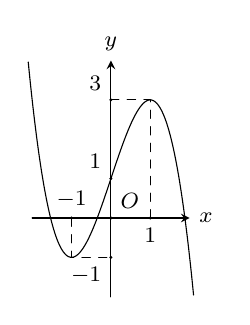
\begin{tikzpicture}[>=stealth,line join=round,line cap=round,font=\footnotesize,scale=0.5]
			\draw[->] (-2,0)--(2,0) node[right] {$x$};
			\draw[->] (0,-2)--(0,4) node[above] {$y$};
			\draw [smooth,domain=-2.1:2.1,samples=100]plot(\x,{-(\x)^3+3*(\x)+1});
			\draw[dashed](-1,0)--(-1,-1)--(0,-1) (1,0)--(1,3)--(0,3);
			\fill (0,0)node[above right]{\footnotesize{$O$}}circle(1.2pt) (1,0)node[below]{\footnotesize{$1$}}circle(1.2pt) (-1,0)node[above]{\footnotesize{$-1$}}circle(1.2pt) (0,1)node[above left]{\footnotesize{$1$}}circle(1.2pt) (0,3)node[above left]{\footnotesize{$3$}}circle(1.2pt)  (0,-1)node[below left]{\footnotesize{$-1$}}circle(1.2pt);
	\end{tikzpicture}}
	\loigiai{Dựa vào đồ thị ta nhận thấy mệnh đề đúng là ``Hàm số đồng biến trên khoảng $(-1;1)$''.}
\end{ex}
\begin{ex}%[Thi Chuyên Đề Lần 4 lớp 12 - THPT Trần Phú - Vĩnh Phúc - 23]%[Phan Anh - EX6-2023]%[2D1Y4-1]
	Đồ thị hàm số $y=\dfrac{2x-3}{x-1}$ có các đường tiệm cận đứng và tiệm cận ngang lần lượt là
	\choice
	{$x=1$ và $y=-3$}
	{\True $x=1$ và $y=2$}
	{$x=2$ và $y=1$}
	{$x=-1$ và $y=2$}
	\loigiai{Ta có $\lim\limits_{x\to+\infty}y=2$ và  $\lim\limits_{x\to-\infty}y=2$ nên đồ thị hàm số nhận $y=2$ làm tiệm cận ngang.\\
		Ta có $\lim\limits_{x\to1^+}y=-\infty$ và $\lim\limits_{x\to1^-}y=+\infty$ nên đồ thị hàm số nhận $x=1$ làm tiệm cận đứng.}
\end{ex}
\begin{ex}%[Thi Chuyên Đề Lần 4 lớp 12 - THPT Trần Phú - Vĩnh Phúc - 23]%[Phan Anh - EX6-2023]%[2H1Y3-2]
	Cho hình chóp tứ giác $S.ABCD$ có đáy $ABCD$ là hình vuông cạnh $a$, cạnh bên $SA$ vuông góc với mặt phẳng đáy và $SA=a\sqrt{2}$. Tính thể tích $V$ của khối chóp $S.ABCD$.
	\choice
	{\True $V=\dfrac{a^3\sqrt{2}}{3}$}
	{$V=\dfrac{a^3\sqrt{2}}{4}$}
	{$V=a^3\sqrt{2}$}
	{$V=\dfrac{a^3\sqrt{2}}{6}$}
	\loigiai{\immini{Do $SA\perp(ABCD)$ nên thể tích của khối chóp là
			$$V=\dfrac{1}{3}\cdot SA\cdot S_{ABCD}=\dfrac{1}{3}\cdot a\sqrt{2}\cdot a^2=\dfrac{a^3\sqrt{2}}{3}.$$}
		{
			\begin{tikzpicture}[>=stealth,line join=round,line cap=round,font=\footnotesize,scale=0.5]
				\path (0,0) coordinate (A)
				(-1.5,-0.8) coordinate (B)
				(4,0) coordinate (D)
				($(B)+(D)-(A)$) coordinate (C)
				($(A)+(0,4)$)coordinate (S)
				;
				\draw (S)--(B)--(C)--(S)--(D)--(C);
				\draw[dashed] (S)--(A)--(B) (D)--(A);
				\foreach \p / \r in {A/135,B/-135,C/-45,S/90,D/45}
				\fill (\p) circle (1.2pt) node[shift={(\r:2mm)}]{$\p$};
	\end{tikzpicture}}}
\end{ex}
\begin{ex}%[Thi Chuyên Đề Lần 4 lớp 12 - THPT Trần Phú - Vĩnh Phúc - 23]%[Phan Anh - EX6-2023]%[2D1Y5-7]
	Đồ thị hàm số $y=\dfrac{2x+1}{x-1}$ cắt trục tung tại điểm có tung độ bằng
	\choice
	{$-\dfrac{1}{2}$}
	{$1$}
	{\True $-1$}
	{$2$}
	\loigiai{Gọi $M$ là giao điểm của đồ thị với trục tung, suy ra $x_M=0$.\\
		Thay vào biểu thức của đồ thị hàm số ta được $y_M=-1$.}
\end{ex}
\begin{ex}%[Thi Chuyên Đề Lần 4 lớp 12 - THPT Trần Phú - Vĩnh Phúc - 23]%[Phan Anh - EX6-2023]%[2D2Y5-1]
	Nghiệm của phương trình $\log_2(2x-6)=3$ là
	\choice
	{$x=6$}
	{$x=9$}
	{$x=8$}
	{\True $x=7$}
	\loigiai{Ta có $\log_2(2x-6)=3\Leftrightarrow2x-6=2^3\Leftrightarrow x=7$.}
\end{ex}
\begin{ex}%[Thi Chuyên Đề Lần 4 lớp 12 - THPT Trần Phú - Vĩnh Phúc - 23]%[Phan Anh - EX6-2023]%[2H3Y2-4]
	Trong KG $Oxyz$, cho mặt phẳng $(P)\colon4x+3y+z-1=0$. Điểm nào dưới đây thuộc $(P)$?
	\choice
	{$M(0;2;-1)$}
	{\True $N(1;1;-6)$}
	{$P(1;-6;1)$}
	{$Q(0;2;1)$}
	\loigiai{Thay tọa độ từng điểm vào phương trình mặt phẳng $(P)$, ta thấy $N\in(P)$.}
\end{ex}
\begin{ex}%[Thi Chuyên Đề Lần 4 lớp 12 - THPT Trần Phú - Vĩnh Phúc - 23]%[Phan Anh - EX6-2023]%[2H3Y1-3]
	Trong KG $Oxyz$, mặt cầu tâm $I(1;0;-2)$ bán kính $R=2$ có phương trình là
	\choice
	{$(x-1)^2+y^2+(z+2)^2=2$}
	{\True $(x-1)^2+y^2+(z+2)^2=4$}
	{$(x+1)^2+y^2+(z-2)^2=4$}
	{$(x+1)^2+y^2+(z-2)^2=2$}
	\loigiai{Phương trình mặt cầu cần tìm là $(x-1)^2+y^2+(z+2)^2=4$.}
\end{ex}
\begin{ex}%[Thi Chuyên Đề Lần 4 lớp 12 - THPT Trần Phú - Vĩnh Phúc - 23]%[Phan Anh - EX6-2023]%[2H2Y1-1]
	Khối nón có bán kính đáy bằng $6$, chiều cao bằng $\dfrac{1}{\pi}$, thể tích $V$ của khối nón bằng
	\choice
	{\True $12$}
	{$2$}
	{$6$}
	{$36$}
	\loigiai{Thể tích của khối nón là $V=\dfrac{1}{3}\pi R^2h=\dfrac{1}{3}\cdot\pi\cdot6^2\cdot\dfrac{1}{\pi}=12$.}
\end{ex}
\begin{ex}%[Thi Chuyên Đề Lần 4 lớp 12 - THPT Trần Phú - Vĩnh Phúc - 23]%[Phan Anh - EX6-2023]%[2D2Y3-1]
	Với $a$, $b$ là hai số thực dương thỏa mãn $\log a=11$, $\log b=13$. Khi đó $\log\left(ab^2\right)$ bằng
	\choice
	{$46$}
	{\True $37$}
	{$180$}
	{$23$}
	\loigiai{Ta có $\log\left(ab^2\right)=\log a+\log b^2=\log a+2\log b=11+2\cdot13=37$.}
\end{ex}
\begin{ex}%[Thi Chuyên Đề Lần 4 lớp 12 - THPT Trần Phú - Vĩnh Phúc - 23]%[Phan Anh - EX6-2023]%[2H3Y1-1]
	Trong không gian tọa độ $Oxyz$, cho các điểm $M(1;2;-3)$ và $N(3;2;4)$. Tọa độ véc-tơ $\overrightarrow{MN}$ là
	\choice
	{$(4;4;1)$}
	{\True $(2;0;7)$}
	{$(-2;0;-7)$}
	{$\left(2;2;\dfrac{1}{2}\right)$}
	\loigiai{Tọa độ của véc-tơ $\overrightarrow{MN}=\left(x_N-x_M;y_N-y_M;z_N-z_M\right)=(2;0;7)$.}
\end{ex}
\begin{ex}%[Thi Chuyên Đề Lần 4 lớp 12 - THPT Trần Phú - Vĩnh Phúc - 23]%[Phan Anh - EX6-2023]%[1D2Y2-1]
	Có bao nhiêu cách chọn ra $2$ học sinh từ một nhóm có $10$ học sinh?
	\choice
	{$90$}
	{$20$}
	{\True $45$}
	{$8$}
	\loigiai{Có $\mathrm{C}_{10}^2=45$ cách chọn $2$ học sinh từ nhóm có $10$ học sinh.}
\end{ex}
\begin{ex}%[Thi Chuyên Đề Lần 4 lớp 12 - THPT Trần Phú - Vĩnh Phúc - 23]%[Phan Anh - EX6-2023]%[2D3Y2-1]
	Biết $F(x)=x^3+C$ là họ nguyên hàm của hàm số $f(x)$ trên tập số thực. Tính tích phân $I=\displaystyle\int\limits_1^3f(x)\mathrm{\,d}x$.
	\choice
	{$23$}
	{$20$}
	{\True $26$}
	{$17$}
	\loigiai{Do $F(x)=x^3+C$ là họ nguyên hàm của hàm số $f(x)$ trên tập số thực nên
		$$I=\displaystyle\int\limits_1^3f(x)\mathrm{\,d}x=x^3\bigg|_1^3=3^3-1^3=26.$$}
\end{ex}
\begin{ex}%[Thi Chuyên Đề Lần 4 lớp 12 - THPT Trần Phú - Vĩnh Phúc - 23]%[Phan Anh - EX6-2023]%[2H3Y1-3]
	Trong KG $Oxyz$, bán kính mặt cầu $(S)\colon x^2+y^2+z^2-2x+2y-4z-2=0$ là
	\choice
	{\True $2\sqrt{2}$}
	{$\sqrt{2}$}
	{$\sqrt{22}$}
	{$4$}
	\loigiai{Ta có $a=1$, $b=-1$, $c=2$, $d=-2\Rightarrow R=\sqrt{a^2+b^2+c^2-d}=2\sqrt{2}$.}
\end{ex}
\begin{ex}%[Thi Chuyên Đề Lần 4 lớp 12 - THPT Trần Phú - Vĩnh Phúc - 23]%[Phan Anh - EX6-2023]%[2D3Y2-3]
	Cho $u$, $v$ là hai hàm số có đạo hàm liên tục trên $[a;b]$. Công thức nào sau đây là đúng?
	\choice
	{$\displaystyle\int\limits_a^bu\mathrm{\,d}v=uv\Big|_a^b+\displaystyle\int\limits_a^bv\mathrm{\,d}u$}
	{$\displaystyle\int\limits_a^bu\mathrm{\,d}v=uv\Big|_a^b-\displaystyle\int\limits_a^bu\mathrm{\,d}v$}
	{$\displaystyle\int\limits_a^bu\mathrm{\,d}v=uv\Big|_a^b$}
	{\True $\displaystyle\int\limits_a^bu\mathrm{\,d}v=uv\Big|_a^b-\displaystyle\int\limits_a^bv\mathrm{\,d}u$}
	\loigiai{Công thức đúng là ``$\displaystyle\int\limits_a^bu\mathrm{\,d}v=uv\Big|_a^b-\displaystyle\int\limits_a^bv\mathrm{\,d}u$''.}
\end{ex}
\begin{ex}%[Thi Chuyên Đề Lần 4 lớp 12 - THPT Trần Phú - Vĩnh Phúc - 23]%[Phan Anh - EX6-2023]%[2D2Y4-2]
	Đạo hàm của hàm số $y=3^{1-x}$ bằng
	\choice
	{$y'=\dfrac{3^{1-x}}{\ln 3}$}
	{$y'=3^{1-x}\ln 3$}
	{$y'=(1-x)3^{-x}$}
	{\True $y'=3^{1-x}\ln \left(\dfrac{1}{3}\right)$}
	\loigiai{Đạo hàm của hàm số là $y'=(1-x)'\cdot3^{1-x}\ln 3=-3^{1-x}\ln 3=3^{1-x}\ln \dfrac{1}{3}$.}
\end{ex}
\begin{ex}%[Thi Chuyên Đề Lần 4 lớp 12 - THPT Trần Phú - Vĩnh Phúc - 23]%[Phan Anh - EX6-2023]%[2D3Y1-1]
	Họ nguyên hàm của hàm số $f(x)=\dfrac{1}{x}+\sin2x$ là
	\choice
	{$\ln x-\dfrac{1}{2}\cos2x+C$}
	{$\ln |x|+\dfrac{1}{2}\cos2x+C$}
	{$-\dfrac{1}{x^2}-\dfrac{1}{2}\cos2x+C$}
	{\True $\ln |x|-\dfrac{1}{2}\cos2x+C$}
	\loigiai{Ta có $\displaystyle\int f(x)\mathrm{\,d}x=\displaystyle\int\left(\dfrac{1}{x}+\sin2x\right)\mathrm{\,d}x=\ln |x|-\dfrac{1}{2}\cos2x+C$.}
\end{ex}
\begin{ex}%[Thi Chuyên Đề Lần 4 lớp 12 - THPT Trần Phú - Vĩnh Phúc - 23]%[Phan Anh - EX6-2023]%[2H1Y3-2]
	Khối lập phương có thể tích bằng $64$ cm$^3$ thì cạnh của hình lập phương đó bằng
	\choice
	{\True $4$ cm}
	{$8$ cm}
	{$6$ cm}
	{$16$ cm}
	\loigiai{Gọi $x$ là cạnh của khối lập phương, ta có $V=x^3\Leftrightarrow x^3=64\Leftrightarrow x=4$ cm.}
\end{ex}
\begin{ex}%[Thi Chuyên Đề Lần 4 lớp 12 - THPT Trần Phú - Vĩnh Phúc - 23]%[Phan Anh - EX6-2023]%[2D2B5-2]
	Phương trình $\left(\sqrt{5}\right)^{x^2+4x+6}=5$ có bao nhiêu nghiệm thực?
	\choice
	{\True $1$}
	{$3$}
	{$2$}
	{$0$}
	\loigiai{Ta có $\left(\sqrt{5}\right)^{x^2+4x+6}=5\Leftrightarrow x^2+4x+6=2\Leftrightarrow x=-2$.\\
		Vậy phương trình có đúng một nghiệm thực.}
\end{ex}
\begin{ex}%[Thi Chuyên Đề Lần 4 lớp 12 - THPT Trần Phú - Vĩnh Phúc - 23]%[Phan Anh - EX6-2023]%[2H3B2-5]
	Trong KG $Oxyz$, cho hai mặt phẳng $(P)\colon x-2y+2z-1=0$ và $(Q)\colon2x+2y-z-3=0$. Gọi $\alpha$ là góc giữa hai mặt phẳng $(P)$ và $(Q)$. Tính giá trị của $\cos\alpha$.
	\choice
	{$-\dfrac{4}{9}$}
	{\True $\dfrac{4}{9}$}
	{$\dfrac{2}{3}$}
	{$-\dfrac{2}{3}$}
	\loigiai{Mặt phẳng $(P)$ và $(Q)$ lần lượt có véc-tơ pháp tuyến là $\overrightarrow{n}_{(P)}=(1;-2;2)$ và  $\overrightarrow{n}_{(Q)}=(2;2;-1)$.\\
		Cosin của góc giữa hai mặt phẳng $(P)$ và $(Q)$ là
		$$\cos\alpha=\dfrac{\left|\overrightarrow{n}_{(P)}\cdot\overrightarrow{n}_{(Q)}\right|}{\left|\overrightarrow{n}_{(P)}\right|\cdot\left|\overrightarrow{n}_{(Q)}\right|}=\dfrac{|2-4-2|}{\sqrt{9}\cdot\sqrt{9}}=\dfrac{4}{9}.$$}
\end{ex}
\begin{ex}%[Thi Chuyên Đề Lần 4 lớp 12 - THPT Trần Phú - Vĩnh Phúc - 23]%[Phan Anh - EX6-2023]%[2D2B6-4]
	Cho hàm số $f(x)=\mathrm{e}^x\cdot2021^{x^2}$. Bất phương trình $f(x)>1$ tương đương với bất phương trình nào bên dưới?
	\choice
	{$x+2x\ln 2021>0$}
	{$x^2\ln 2021>0$}
	{\True $x+x^2\ln 2021>0$}
	{$1+x^2\ln 2021>0$}
	\loigiai{Ta có $f(x)>1\Leftrightarrow\mathrm{e}^x\cdot2021^{x^2}>1\Leftrightarrow\ln \left(\mathrm{e}^x\cdot2021^{x^2}\right)>\ln 1\Leftrightarrow x+x^2\ln 2021>0$.}
\end{ex}
\begin{ex}%[Thi Chuyên Đề Lần 4 lớp 12 - THPT Trần Phú - Vĩnh Phúc - 23]%[Phan Anh - EX6-2023]%[2D3B1-2]
	Tính nguyên hàm của hàm số $f(x)=\dfrac{\mathrm{e}^{2x}}{\mathrm{e}^x+2}$.
	\choice
	{$F(x)=\mathrm{e}^{2x}-4\ln \left(\mathrm{e}^x+2\right)+C$}
	{$F(x)=\mathrm{e}^x+2\ln \left(\mathrm{e}^x+2\right)+C$}
	{\True $F(x)=\mathrm{e}^x-2\ln \left(\mathrm{e}^x+2\right)+C$}
	{$F(x)=\ln \left(\mathrm{e}^x+2\right)+C$}
	\loigiai{Ta có $F(x)=\displaystyle\int f(x)\mathrm{\,d}x=\displaystyle\int\dfrac{\mathrm{e}^{2x}}{\mathrm{e}^x+2}\mathrm{\,d}x$.\\
		Đặt $t=\mathrm{e}^x$, $\mathrm{\,d}t=\mathrm{e}^x\mathrm{\,d}x$. Khi đó ta có 
		$$F(x)=\displaystyle\int\dfrac{t}{t+2}\mathrm{\,d}t=\displaystyle\int\left(1-\dfrac{2}{t+2}\right)\mathrm{\,d}t=t-2\ln |t+2|+C=\mathrm{e}^x-2\ln \left(\mathrm{e}^x+2\right)+C.$$}
\end{ex}
\begin{ex}%[Thi Chuyên Đề Lần 4 lớp 12 - THPT Trần Phú - Vĩnh Phúc - 23]%[Phan Anh - EX6-2023]%[2D1B2-2]
	Cho hàm số $y=f(x)$ liên tục trên $\mathbb{R}$ và có bảng xét dấu đạo hàm như bên dưới
	\begin{center}
		\begin{center}
			
\begin{tikzpicture}[scale=1, font=\footnotesize, line join=round, line cap=round, >=stealth]
				\tkzTabInit[nocadre=false, lgt=1.2, espcl=1.8, deltacl=0.6]
				{$x$/0.7, $f'(x)$/0.7}
				{$-\infty$,$-3$,$1$,$2$,$+\infty$}
				\tkzTabLine{,-,0,+,0,+,0,-,}
			\end{tikzpicture}
		\end{center}
	\end{center}
	Điểm cực đại của hàm số là
	\choice
	{$x=0$}
	{$x=-3$}
	{$x=1$}
	{\True $x=2$}
	\loigiai{Từ bảng xét dấu của đạo hàm, ta có bảng biến thiên của hàm số là
		\begin{center}
			
\begin{tikzpicture}[scale=1, font=\footnotesize, line join=round, line cap=round, >=stealth]
				\tkzTabInit[nocadre=false, lgt=1.2, espcl=1.8, deltacl=0.6]
				{$x$/0.7, $f'(x)$/0.7,$f(x)$/2.2}
				{$-\infty$,$-3$,$1$,$2$,$+\infty$}
				\tkzTabLine{,-,0,+,0,+,0,-,}
				\tkzTabVar{+/,-/,R,+/,-/}
			\end{tikzpicture}
		\end{center}
		Vậy điểm cực đại của hàm số là $x=2$.}
\end{ex}
\begin{ex}%[Thi Chuyên Đề Lần 4 lớp 12 - THPT Trần Phú - Vĩnh Phúc - 23]%[Phan Anh - EX6-2023]%[2D1B1-1]
	Hàm số nào dưới đây đồng biến trên $\mathbb{R}$?
	\choice
	{$y=x^3-3x^2-1$}
	{\True $y=x^3-x^2+6x-1$}
	{$y=\dfrac{x-2}{x+1}$}
	{$y=x^4+2x^2-1$}
	\loigiai{Xét hàm số $y=x^3-x^2+6x-1$ có $y'=3x^2-2x+6=2x^2+(x-1)^2+5>0$, $\forall x\in\mathbb{R}$.\\
		Vậy hàm số $y=x^3-x^2+6x-1$ đồng biến trên $\mathbb{R}$.}
\end{ex}
\begin{ex}%[Thi Chuyên Đề Lần 4 lớp 12 - THPT Trần Phú - Vĩnh Phúc - 23]%[Phan Anh - EX6-2023]%[2H2B1-2]
	Cho hình trụ có diện tích xung quanh bằng $50\pi$ và độ dài đường sinh bằng đường kính của đường tròn đáy. Tính bán kính $r$ của đường tròn đáy.
	\choice
	{\True $r=\dfrac{5\sqrt{2}}{2}$}
	{$r=5\sqrt{\pi}$}
	{$r=\dfrac{5\sqrt{2\pi}}{2}$}
	{$r=5$}
	\loigiai{Do độ dài đường sinh bằng đường kính của đường tròn đáy nên $h=2r$.\\
		Ta có $S_{\text{xq}}=2\pi rh=50\pi\Leftrightarrow 2r^2=25\Leftrightarrow r=\dfrac{5\sqrt{2}}{2}$.}
\end{ex}
\begin{ex}%[Thi Chuyên Đề Lần 4 lớp 12 - THPT Trần Phú - Vĩnh Phúc - 23]%[Phan Anh - EX6-2023]%[2D3B2-1]
	Nếu $\displaystyle\int\limits_1^4f(x)\mathrm{\,d}x=-2$ và $\displaystyle\int\limits_1^4g(x)\mathrm{\,d}x=-6$ thì $\displaystyle\int\limits_1^4\left[2f(x)-g(x)+1\right]\mathrm{\,d}x$ bằng
	\choice
	{$2$}
	{$-4$}
	{\True $5$}
	{$3$}
	\loigiai{Ta có $\displaystyle\int\limits_1^4\left[2f(x)-g(x)+1\right]\mathrm{\,d}x=2\displaystyle\int\limits_1^4f(x)\mathrm{\,d}x-\displaystyle\int\limits_1^4g(x)\mathrm{\,d}x+x\bigg|_1^4=2\cdot(-2)-(-6)+(4-1)=5$.}
\end{ex}
\begin{ex}%[Thi Chuyên Đề Lần 4 lớp 12 - THPT Trần Phú - Vĩnh Phúc - 23]%[Phan Anh - EX6-2023]%[2D3B2-1]
	Cho $\displaystyle\int\limits_{-1}^2f(t)\mathrm{\,d}t=2$ và $\displaystyle\int\limits_{-1}^2g(x)\mathrm{\,d}x=-1$. Tính $\displaystyle\int\limits_{-1}^2\left[x+2f(x)-3g(x)\right]\mathrm{\,d}x$.
	\choice
	{\True $\dfrac{17}{2}$}
	{$\dfrac{7}{2}$}
	{$\dfrac{5}{2}$}
	{$\dfrac{11}{2}$}
	\loigiai{Ta có $\displaystyle\int\limits_{-1}^2\left[x+2f(x)-3g(x)\right]\mathrm{\,d}x=\dfrac{x^2}{2}\Bigg|_{-1}^2+2\displaystyle\int\limits_{-1}^2f(x)\mathrm{\,d}x-3\displaystyle\int\limits_{-1}^2g(x)\mathrm{\,d}x=\dfrac{3}{2}+2\cdot2-3\cdot(-1)=\dfrac{17}{2}$.}
\end{ex}
\begin{ex}%[Thi Chuyên Đề Lần 4 lớp 12 - THPT Trần Phú - Vĩnh Phúc - 23]%[Phan Anh - EX6-2023]%[2D1B5-1]
	\immini{Đường cong trong hình vẽ bên là đồ thị của hàm số nào trong các hàm số sau
		\choice
		{$y=x^4+2x^2$}
		{$y=x^4-2x^2+2$}
		{$y=-x^4+2x^2-2$}
		{\True $y=x^4-2x^2-2$}}
	{
		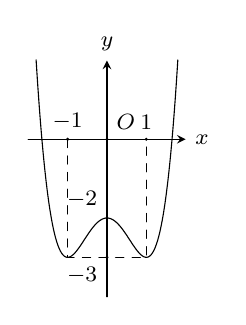
\begin{tikzpicture}[>=stealth,line join=round,line cap=round,font=\footnotesize,scale=0.5]
			\draw[->] (-2,0)--(2,0) node[right] {$x$};
			\draw[->] (0,-4)--(0,2) node[above] {$y$};
			\draw [smooth,domain=-1.8:1.8,samples=100]plot(\x,{(\x)^4-2*(\x)^2-2});
			\draw[dashed](-1,0)--(-1,-3)--(1,-3)--(1,0);
			\fill (0,0)node[above right]{\footnotesize{$O$}}circle(1.2pt) (1,0)node[above]{\footnotesize{$1$}}circle(1.2pt) (-1,0)node[above]{\footnotesize{$-1$}}circle(1.2pt) (0,-2)node[above left]{\footnotesize{$-2$}}circle(1.2pt) (0,-3)node[below left]{\footnotesize{$-3$}}circle(1.2pt);
	\end{tikzpicture}}
	\loigiai{Đồ thị đề bài là đồ thị của hàm số trùng phương bậc bốn, hệ số $a>0$ và cắt $Oy$ tại điểm $(0;-2)$. Suy ra hàm số thỏa mãn bài toán là $y=x^4-2x^2-2$.}
\end{ex}
\begin{ex}%[Thi Chuyên Đề Lần 4 lớp 12 - THPT Trần Phú - Vĩnh Phúc - 23]%[Phan Anh - EX6-2023]%[2H3B1-3]
	Trong KG $Oxyz$, cho hai điểm $A(1;2;2)$ và $B(0;2;1)$. Mặt cầu có tâm thuộc trục $Ox$ và đi qua hai điểm $A$, $B$ có đường kính bằng
	\choice
	{$\sqrt{2}$}
	{$3$}
	{\True $6$}
	{$2$}
	\loigiai{Gọi $I(a;0;0)\in Ox$ là tâm mặt cầu cần tìm.\\
		Ta có $IA=IB\Leftrightarrow(a-1)^2+4+4=a^2+4+1\Leftrightarrow a=2$.\\
		Vậy tâm $I(2;0;0)$, suy ra $R=IA=3$, nên đường kính của mặt cầu là $d=2R=6$.}
\end{ex}
\begin{ex}%[Thi Chuyên Đề Lần 4 lớp 12 - THPT Trần Phú - Vĩnh Phúc - 23]%[Phan Anh - EX6-2023]%[2D3B2-4]
	Cho hàm số $f(x)$ liên tục trên $[-1;+\infty)$ và $\displaystyle\int\limits_0^3f\left(\sqrt{x+1}\right)\mathrm{\,d}x=8$. Tính tích phân $I=\displaystyle\int\limits_1^2xf(x)\mathrm{\,d}x$
	\choice
	{\True $I=4$}
	{$I=-4$}
	{$I=\dfrac{1}{4}$}
	{$I=-\dfrac{1}{4}$}
	\loigiai{Đặt $t=\sqrt{x+1}\Rightarrow t^2=x+1\Rightarrow2t\mathrm{\,d}t=\mathrm{\,d}x$.\\
		Với $x=0\Rightarrow t=1$, $x=3\Rightarrow t=2$.\\
		Ta có $\displaystyle\int\limits_0^3f\left(\sqrt{x+1}\right)\mathrm{\,d}x=8\Leftrightarrow\displaystyle\int\limits_1^2f(t)2t\mathrm{\,d}t=8\Leftrightarrow\displaystyle\int\limits_1^2tf(t)\mathrm{\,d}t=4$.\\
		Vậy $I=\displaystyle\int\limits_1^2xf(x)\mathrm{\,d}x=4$.}
\end{ex}
\begin{ex}%[Thi Chuyên Đề Lần 4 lớp 12 - THPT Trần Phú - Vĩnh Phúc - 23]%[Phan Anh - EX6-2023]%[2D3B3-7]
	Một ô-tô đang chạy thì người lái đạp phanh. Từ thời điểm đó, ô-tô chuyển động chậm dần đều với vận tốc $v(t)=-12t+24$ m/s, trong đó $t$ là khoảng thời gian tính bằng giây, kể từ lúc bắt đầu đạp phanh. Hỏi từ lúc đạp phanh đến khi dừng hẳn, ô-tô di chuyển bao nhiêu mét?
	\choice
	{$15$ m}
	{\True $24$ m}
	{$20$ m}
	{$18$ m}
	\loigiai{Khi ô-tô dừng hẳn thì $v(t)=0\Leftrightarrow-12t+24=0\Leftrightarrow t=2$.\\
		Đoạn đường ô-tô di chuyển được là $S=\displaystyle\int\limits_0^2v(t)\mathrm{\,d}t=\displaystyle\int\limits_0^2(-12t+24)\mathrm{\,d}t=\left(-6t^2+24t\right)\bigg|_0^2=24$ m.}
\end{ex}
\begin{ex}%[Thi Chuyên Đề Lần 4 lớp 12 - THPT Trần Phú - Vĩnh Phúc - 23]%[Phan Anh - EX6-2023]%[1H3B3-3]
	Cho hình chóp $S.ABCD$ có đáy $ABCD$ là hình vuông cạnh bằng $2$, $SA$ vuông góc với mặt phẳng $(ABCD)$ và $SA=2\sqrt{2}$. Góc giữa $SC$ với mặt phẳng $(ABCD)$ là
	\choice
	{\True $45^\circ$}
	{$60^\circ$}
	{$30^\circ$}
	{$90^\circ$}
	\loigiai{\immini{Do $SA\perp(ABCD)$ nên $AC$ là hình chiếu của $SC$ lên $(ABCD)$.\\
			Góc giữa $SC$ với $(ABCD)$ là góc $\widehat{SCA}$.\\
			Xét tam giác $SAC$ ta có $\tan\widehat{SCA}=\dfrac{SA}{AC}=\dfrac{2\sqrt{2}}{2\sqrt{2}}=1\Rightarrow\widehat{SCA}=45^\circ$.\\
			Vậy góc giữa $SC$ với $(ABCD)$ bằng $45^\circ$.}
		{
			\begin{tikzpicture}[>=stealth,line join=round,line cap=round,font=\footnotesize,scale=0.5]
				\path (0,0) coordinate (A)
				(-2.5,-1.4) coordinate (B)
				(6,0) coordinate (D)
				($(B)+(D)-(A)$) coordinate (C)
				($(A)+(0,6)$)coordinate (S)
				;
				\draw (S)--(B)--(C)--(S)--(D)--(C);
				\draw[dashed] (S)--(A)--(B) (D)--(A)--(C);
				\foreach \p / \r in {A/135,B/-135,C/-45,S/90,D/45}
				\fill (\p) circle (1.2pt) node[shift={(\r:2mm)}]{$\p$};
	\end{tikzpicture}}}
\end{ex}
\begin{ex}%[Thi Chuyên Đề Lần 4 lớp 12 - THPT Trần Phú - Vĩnh Phúc - 23]%[Phan Anh - EX6-2023]%[2D2B6-3]
	Có bao nhiêu giá trị nguyên của $m$ để bất phương trình $\log_3^2x+m\log_3x\ge m$ nghiệm đúng với mọi giá trị của $x\in(0;+\infty)$.
	\choice
	{$7$}
	{$6$}
	{$4$}
	{\True $5$}
	\loigiai{Đặt $t=\log_3x$, với $x\in(0;+\infty)$ thì $t\in\mathbb{R}$. Yêu cầu bài toán trở thành
		$$t^2+mt-m\ge0,\forall t\in\mathbb{R}\Leftrightarrow\Delta=m^2+4m\le0\Leftrightarrow-4\le m\le0.$$
		Do $m$ là số nguyên nên $m\in\{-4;-3;-2;-1;0\}$, vậy có $5$ giá trị $m$ thỏa bài toán.}
\end{ex}
\begin{ex}%[Thi Chuyên Đề Lần 4 lớp 12 - THPT Trần Phú - Vĩnh Phúc - 23]%[Phan Anh - EX6-2023]%[2D3B2-1]
	Tích phân $\displaystyle\int\limits_0^1\dfrac{1}{x^2+4x+3}\mathrm{\,d}x$ có kết quả là
	\choice
	{$\dfrac{1}{3}\ln \dfrac{3}{2}$}
	{\True $\dfrac{1}{2}\ln \dfrac{3}{2}$}
	{$-\dfrac{1}{2}\ln \dfrac{3}{2}$}
	{$\ln \dfrac{3}{2}$}
	\loigiai{Ta có
		\begin{eqnarray*}
			&&\displaystyle\int\limits_0^1\dfrac{1}{x^2+4x+3}\mathrm{\,d}x=\dfrac{1}{2}\cdot\displaystyle\int\limits_0^1\left(\dfrac{1}{x+1}-\dfrac{1}{x+3}\right)\mathrm{\,d}x\\
			&=&\dfrac{1}{2}\left(\ln |x+1|-\ln |x+3|\right)\bigg|_0^1=\dfrac{1}{2}(\ln 2-\ln 4-\ln 1+\ln 3)=\dfrac{1}{2}\ln \dfrac{3}{2}.
	\end{eqnarray*}}
\end{ex}
\begin{ex}%[Thi Chuyên Đề Lần 4 lớp 12 - THPT Trần Phú - Vĩnh Phúc - 23]%[Phan Anh - EX6-2023]%[1D2K5-2]
	Có $30$ chiếc thẻ được đánh số từ $1$ đến $30$. Chọn ngẫu nhiên $2$ thẻ. Xác suất để chọn được ít nhất một thẻ đánh số nguyên tố bằng
	\choice
	{\True $0{,}56$}
	{$0{,}41$}
	{$0{,}46$}
	{$0{,}52$}
	\loigiai{Chọn ngẫu nhiên $2$ thẻ tùy ý, ta có $\mathrm{C}_{30}^2$ cách chọn.\\
		Từ $1$ đến $30$ có $10$ số nguyên tố, để chọn được cả hai thẻ đều không phải là số nguyên tố, ta có $\mathrm{C}_{20}^2$ cách.\\
		Vậy để có ít nhất một trong hai thẻ là số nguyên tố, thì ta có $\mathrm{C}_{30}^2-\mathrm{C}_{20}^2$ cách.\\
		Xác suất để trong hai thẻ được chọn có ít nhất một thẻ đánh số nguyên tố là $\mathrm{P}=\dfrac{\mathrm{C}_{30}^2-\mathrm{C}_{20}^2}{\mathrm{C}_{30}^2}=\dfrac{49}{87}\approx0{,}56$.}
\end{ex}
\begin{ex}%[Thi Chuyên Đề Lần 4 lớp 12 - THPT Trần Phú - Vĩnh Phúc - 23]%[Phan Anh - EX6-2023]%[2D3K2-4]
	Xét hàm số $f(x)$ liên tục trên đoạn $[0;1]$ và thỏa mãn điều kiện
	$$4xf\left(x^2\right)+3f(1-x)=\sqrt{1-x^2},\quad\forall x\in[0;1].$$
	Tích phân $I=\displaystyle\int\limits_0^1f(x)\mathrm{\,d}x$ bằng
	\choice
	{$I=\dfrac{\pi}{4}$}
	{$I=\dfrac{\pi}{6}$}
	{$I=\dfrac{\pi}{16}$}
	{\True $I=\dfrac{\pi}{20}$}
	\loigiai{Lấy tích phân từ $0$ đến $1$ hai vế của giả thiết ta được
		$$4\displaystyle\int\limits_0^1xf\left(x^2\right)\mathrm{\,d}x+3\displaystyle\int\limits_0^1f(1-x)\mathrm{\,d}x=\displaystyle\int\limits_0^1\sqrt{1-x^2}\mathrm{\,d}x.\qquad(*)$$
		\begin{itemize}
			\item Đặt $t=x^2$, $\mathrm{\,d}t=2x\mathrm{\,d}x$.\\
			Với $x=0\Rightarrow t=0$, $x=1\Rightarrow t=1$. Ta có 
			$$\displaystyle\int\limits_0^1xf\left(x^2\right)\mathrm{\,d}x=\dfrac{1}{2}\displaystyle\int\limits_0^1f(t)\mathrm{\,d}t=\dfrac{1}{2}\displaystyle\int\limits_0^1f(x)\mathrm{\,d}x=\dfrac{1}{2}I.$$
			\item Đặt $t=1-x$, $\mathrm{\,d}t=-\mathrm{\,d}x$.\\
			Với $x=0\Rightarrow t=1$, $x=1\Rightarrow t=0$. Ta có 
			$$\displaystyle\int\limits_0^1f(1-x)\mathrm{\,d}x=-\displaystyle\int\limits_1^0f(t)\mathrm{\,d}t=\displaystyle\int\limits_0^1f(t)\mathrm{\,d}t=\displaystyle\int\limits_0^1f(x)\mathrm{\,d}x=I.$$
			\item Đặt $x=\sin t$ với $t\in\left[-\dfrac{\pi}{2};\dfrac{\pi}{2}\right]$, $\mathrm{\,d}x=\cos t\mathrm{\,d}t$.\\
			Với $x=0\Rightarrow t=0$, $x=1\Rightarrow t=\dfrac{\pi}{2}$. Ta có 
			$$\displaystyle\int\limits_0^1\sqrt{1-x^2}\mathrm{\,d}x=\displaystyle\int\limits_0^{\tfrac{\pi}{2}}\sqrt{1-\sin^2t}\cos t\mathrm{\,d}t=\displaystyle\int\limits_0^{\tfrac{\pi}{2}}\cos^2t\mathrm{\,d}t=\displaystyle\int\limits_0^{\tfrac{\pi}{2}}\dfrac{1+\cos2x}{2}\mathrm{\,d}t=\left(\dfrac{x}{2}+\dfrac{\sin2x}{4}\right)\Bigg|_0^{\tfrac{\pi}{2}}=\dfrac{\pi}{4}.$$
		\end{itemize}
		Do đó, $(*)\Leftrightarrow2I+3I=\dfrac{\pi}{4}\Leftrightarrow I=\dfrac{\pi}{20}$.}
\end{ex}
\begin{ex}%[Thi Chuyên Đề Lần 4 lớp 12 - THPT Trần Phú - Vĩnh Phúc - 23]%[Phan Anh - EX6-2023]%[1H3K5-3]
	\immini{Cho hình chóp tứ giác đều $S.ABCD$ có tất cả các cạnh bằng $2$. Khoảng cách từ $A$ đến mặt phẳng $(SCD)$ bằng
		\choice
		{$\sqrt{2}$}
		{$\sqrt{3}$}
		{$\dfrac{\sqrt{6}}{3}$}
		{\True $\dfrac{2\sqrt{6}}{3}$}}
	{
		\begin{tikzpicture}[>=stealth,line join=round,line cap=round,font=\footnotesize,scale=0.5]
			\path (0,0) coordinate (A)
			(-2.5,-1.4) coordinate (B)
			(6,0) coordinate (D)
			($(B)+(D)-(A)$) coordinate (C)
			($(A)!0.5!(C)$) coordinate (O)
			($(O)+(0,6)$)coordinate (S)
			;
			\draw (S)--(B)--(C)--(S)--(D)--(C);
			\draw[dashed] (S)--(A)--(B) (D)--(A);
			\foreach \p / \r in {A/135,B/-135,C/-45,S/90,D/45}
			\fill (\p) circle (1.2pt) node[shift={(\r:2mm)}]{$\p$};
	\end{tikzpicture}}
	\loigiai{\immini{Gọi $O$ là trung điểm của $AC$, suy ra $\mathrm{d}(A,(SCD))=2\mathrm{d}(O,(SCD))$.\\
			Do $S.ABCD$ là hình chóp tứ giác đều nên $SO\perp(ABCD)$, suy ra $SO\perp CD$.\\
			Kẻ $OM\perp CD$ tại $M$, suy ra $CD\perp (SOM)$.\\
			Do $CD\subset(SCD)$ nên $(SCD)\perp(SOM)$ theo giao tuyến $SM$.\\
			Kẻ $OH\perp SM$ tại $H$ trong $(SOM)$, suy ra $OH\perp(SCD)$.\\
			Vậy $\mathrm{d}(O,(SCD))=OH$.\\
			Tam giác $SAO$ có $SO^2=SA^2-AO^2=2$.}
		{
			\begin{tikzpicture}[>=stealth,line join=round,line cap=round,font=\footnotesize,scale=0.55]
				\path (0,0) coordinate (A)
				(-2.5,-1.4) coordinate (B)
				(6,0) coordinate (D)
				($(B)+(D)-(A)$) coordinate (C)
				($(A)!0.5!(C)$) coordinate (O)
				($(O)+(0,6)$)coordinate (S)
				($(D)!0.5!(C)$) coordinate (M)
				($(S)!0.7!(M)$) coordinate (H)
				;
				\draw (M)--(S)--(B)--(C)--(S)--(D)--(C);
				\draw[dashed] (M)--(O)--(S)--(A)--(B)--(D)--(A)--(C) (O)--(H);
				\foreach \p / \r in {A/135,B/-135,C/-45,S/90,D/45,O/-90,M/-45,H/45}
				\fill (\p) circle (1.2pt) node[shift={(\r:2mm)}]{$\p$};
		\end{tikzpicture}}
		\noindent
		Xét tam giác $SOM$, ta có $\dfrac{1}{OH^2}=\dfrac{1}{SO^2}+\dfrac{1}{OM^2}=\dfrac{1}{2}+\dfrac{1}{1}=\dfrac{3}{2}$.\\
		Suy ra $\mathrm{d}(O,(SCD))=OH=\dfrac{\sqrt{6}}{3}$, vậy $\mathrm{d}(A,(SCD))=2\mathrm{d}(O,(SCD))=\dfrac{2\sqrt{6}}{3}$.}
\end{ex}
\begin{ex}%[Thi Chuyên Đề Lần 4 lớp 12 - THPT Trần Phú - Vĩnh Phúc - 23]%[Phan Anh - EX6-2023]%[2H2K1-4]
	Một thùng hình trụ có bán kính đáy bằng $2$ m, bên trong thùng có chứa một lượng nước. Biết rằng khi để thùng nằm ngang thì phần bề mặt nước là một hình vuông, mặt nước nằm dưới trục hình trụ và cách trục của hình trụ một khoảng bằng $\sqrt{3}$ (m). Nếu để thùng thẳng đứng thì chiều cao của nước trong thùng bằng
	\choice
	{$10{,}67$ cm}
	{\True $5{,}77$ cm}
	{$33{,}3$ cm}
	{$8{,}33$ cm}
	\loigiai{\immini{Từ giả thiết bài toán ta suy ra phần bề mặt nước là thiết diện song song với trục hình trụ và cách trục hình trụ một khoảng bằng $\sqrt{3}$ m. Gọi thiết diện đó là $ABCD$ như hình vẽ.\\
			Gọi $H$ là hình chiếu của $O$ lên $AB$, ta có $OH=\sqrt{3}$.\\
			Xét tam giác $OAH$, ta có $AH=\sqrt{OA^2-OH^2}=\sqrt{4-3}=1$.\\
			Suy ra chiều cao của hình trụ là $AD=AB=2AH=2$ m.\\
			Nhận thấy rằng $\triangle OAB$ đều, do đó, diện tích phần hình viên phân cung nhỏ $AB$ là
			$$S=\dfrac{1}{6}S_{\text{đáy}}-S_{OAB}=\dfrac{1}{6}\cdot4\pi-\dfrac{2^2\sqrt{3}}{4}=\dfrac{2\pi}{3}-\sqrt{3}.$$}
		{
			\begin{tikzpicture}[>=stealth,line join=round,line cap=round,font=\footnotesize,scale=0.45]
				\tkzDefPoints{0/0/O, 0/7/O'}
				\def\a{5}
				\def\b{1.5}
				\def\x{-80}
				\def\y{40}
				\path (0,0) coordinate (O)
				(0,7) coordinate (O')
				($(O)+({\a*cos(\x)},{\b*sin(\x)})$) coordinate (A)
				($(O)+({\a*cos(\y)},{\b*sin(\y)})$) coordinate (B)
				($(O)+({\a*cos(\y)},{\b*sin(\y)+7})$) coordinate (C)
				($(O)+({\a*cos(\x)},{\b*sin(\x)+7})$) coordinate (D)
				($(A)!0.5!(B)$) coordinate (H)
				;
				\draw[smooth,dashed,samples=200,variable=\t,domain=0:180] plot({\a*cos (\t)},{\b*sin(\t)});
				\draw[smooth,samples=200,variable=\t,domain=0:-180] plot({\a*cos (\t)},{\b*sin(\t)});
				\draw[smooth,samples=200,variable=\t,domain=0:360] plot({\a*cos (\t)},{\b*sin(\t)+7});
				\draw (-5,0)--(-5,7) (5,0)--(5,7);
				\draw (C)--(D)--(A);
				\draw[dashed] (O')--(O)--(H) (O)--(A)--(B)--(C);
				\foreach \p / \r in {A/-135,B/45,C/45,D/135,O/-135,O'/135,H/-45}
				\fill (\p) circle (1.2pt) node[shift={(\r:2mm)}]{$\p$};
		\end{tikzpicture}}
		\noindent
		Thể tích nước trong thùng là $V_{\text{nước}}=S\cdot h=\dfrac{4\pi}{3}-2\sqrt{3}$.\\
		Khi để thùng thẳng đứng thì chiều cao cột nước là $h_{\text{nước}}=\dfrac{V_{\text{nước}}}{S_{\text{đáy}}}=\dfrac{\dfrac{4\pi}{3}-2\sqrt{3}}{4\pi}\approx0{,}0577$ (m)}
\end{ex}
\begin{ex}%[Thi Chuyên Đề Lần 4 lớp 12 - THPT Trần Phú - Vĩnh Phúc - 23]%[Phan Anh - EX6-2023]%[2H3K4-1]
	Cho hình chóp $S.ABCD$ có $ABCD$ là hình vuông cạnh bằng $4$, $SA$ vuông góc với đáy. Góc giữa $SC$ và mặt $(SBD)$ bằng $\alpha$. Biết $\cos\alpha=\dfrac{3\sqrt{10}}{10}$ và tam giác $SAC$ không cân. Thể tích khối chóp $S.ABCD$ bằng
	\choice
	{\True $\dfrac{32\sqrt{2}}{3}$}
	{$\dfrac{128}{3}$}
	{$\dfrac{16}{3}$}
	{$\dfrac{16\sqrt{2}}{3}$}
	\loigiai{\immini{Xét hình chóp trong hệ tọa độ $Oxyz$, sao cho $A$ trùng với gốc tọa độ $O$, các đỉnh $B$, $D$, $S$ lần lượt thuộc các trục tọa độ như hình vẽ.\\
			Ta có $A(0;0;0)$, $B(4;0;0)$, $D(0;4;0)$, $S(0;0;h)$, $h>0$.\\
			Do $ABCD$ là hình vuông nên $C(4;4;0)$, $\overrightarrow{SC}=(4;4;-h)$.\\
			Ta có $\heva{&\overrightarrow{SB}=(4;0;-h)\\&\overrightarrow{SD}=(0;4;-h)}\Rightarrow\overrightarrow{n}_{(SBD)}=\left[\overrightarrow{SB},\overrightarrow{SD}\right]=(4h;4h;16)$.\\
			Xét $\alpha$ là góc giữa $SC$ và $(SBD)$, ta có $$\sin\alpha=\dfrac{\left|\overrightarrow{SC}\cdot\overrightarrow{n}_{(SBD)}\right|}{\left|\overrightarrow{SC}\right|\cdot\left|\overrightarrow{n}_{(SBD)}\right|}\Leftrightarrow\dfrac{1}{\sqrt{10}}=\dfrac{16h}{\sqrt{32+h^2}\cdot\sqrt{32h^2+256}}$$}
		{
			\begin{tikzpicture}[>=stealth,line join=round,line cap=round,font=\footnotesize,scale=0.5]
				\path (0,0) coordinate (A)
				(-2.5,-1.6) coordinate (B)
				(6,0) coordinate (D)
				($(B)+(D)-(A)$) coordinate (C)
				($(A)+(0,6)$)coordinate (S)
				($(A)!1.3!(B)$) coordinate (x)
				($(A)!1.3!(D)$) coordinate (y)
				($(A)!1.3!(S)$) coordinate (z)
				;
				\draw (S)--(B)--(C)--(S)--(D)--(C);
				\draw[dashed] (S)--(A)--(B) (D)--(A);
				\draw[->](B)--(x);
				\draw[->](D)--(y);
				\draw[->](S)--(z);
				\foreach \p / \r in {A/135,B/135,C/-45,S/135,D/45}
				\fill (\p) circle (1.2pt) node[shift={(\r:2mm)}]{$\p$};
				\foreach \k / \h in {x/-135,y/45,z/90}
				\fill (\k) node[shift={(\h:2mm)}]{$\k$};
		\end{tikzpicture}}
		$\Leftrightarrow32\left(32+h^2\right)\left(h^2+8\right)=2560h^2\Leftrightarrow h^4-40h^2+256=0\Leftrightarrow\hoac{&h^2=32\\&h^2=8}\Leftrightarrow\hoac{&h=4\sqrt{2}\text{ (loại vì }AC=4\sqrt{2})\\&h=2\sqrt{2}.}$\\
		Vậy thể tích của khối chóp $S.ABCD$ là $V=\dfrac{1}{3}\cdot SA\cdot S_{ABCD}=\dfrac{1}{3}\cdot2\sqrt{2}\cdot4^2=\dfrac{32\sqrt{2}}{3}$.}
\end{ex}
\begin{ex}%[Thi Chuyên Đề Lần 4 lớp 12 - THPT Trần Phú - Vĩnh Phúc - 23]%[Phan Anh - EX6-2023]%[2D1K3-1]
	Cho hàm số $y=f(x)$ có đạo hàm $f'(x)=(x+1)(x-1)^2(x-2)$. Giá trị nhỏ nhất của hàm số $y=f(2x+1)+\dfrac{8}{3}x^3+4x^2-\dfrac{5}{3}$, $x\in\left[-1;\dfrac{1}{2}\right]$ bằng
	\choice
	{$f(0)-1$}
	{\True $f(1)-\dfrac{5}{3}$}
	{$f(-1)-\dfrac{1}{3}$}
	{$f(2)-\dfrac{1}{3}$}
	\loigiai{Ta có $y'=2f'(2x+1)+8x^2+8x=2\left[f'(2x+1)+4x^2+4x\right]$.\\
		Từ giả thiết ta suy ra $y'=2\left[(2x+2)(2x)^2(2x-1)+2x(2x+2)\right]=4x(2x+2)\left(4x^2-2x+1\right)$.\\
		Ta có $y'=0\Leftrightarrow\hoac{&x=0\\&x=-1}$. Xét trên $\left[-1;\dfrac{1}{2}\right]$, bảng biến thiên của hàm số như hình vẽ bên dưới.
		\begin{center}
			
\begin{tikzpicture}[scale=1, font=\footnotesize, line join=round, line cap=round, >=stealth]
				\tkzTabInit[nocadre=false, lgt=1.2, espcl=3.2, deltacl=0.6]
				{$x$/1, $y'$/0.7,$y$/2.2}
				{$-1$,$0$,$\dfrac{1}{2}$}
				\tkzTabLine{,-,0,+,}
				\tkzTabVar{+/$ $,-/$ $,+/$ $}
			\end{tikzpicture}
		\end{center}
		Từ bảng biến thiên, suy ra giá trị nhỏ nhất của hàm số trên $\left[-1;\dfrac{1}{2}\right]$ là $y(0)=f(1)-\dfrac{5}{3}$.}
\end{ex}
\begin{ex}%[Thi Chuyên Đề Lần 4 lớp 12 - THPT Trần Phú - Vĩnh Phúc - 23]%[Phan Anh - EX6-2023]%[2D2G5-5]
	Có bao nhiêu số nguyên dương $a$ để tồn tại đúng hai số thực $b$ phân biệt, thỏa mãn điều kiện $$\left(4\log_2^2b+\log_2b-5\right)\sqrt{7^b-a}=0.$$
	\choice
	{$48$}
	{$47$}
	{$49$}
	{\True $46$}
	\loigiai{Điều kiện: $\heva{&b>0\\&7^b-a\ge0}$. Biến đổi giả thiết bài toán ta được
		$$\left(4\log_2^2b+\log_2b-5\right)\sqrt{7^b-a}=0\Leftrightarrow\hoac{&4\log_2^2b+\log_2b-5=0\\&7^b-a=0}\Leftrightarrow\hoac{&\log_2b=1\\&\log_2b=-\dfrac{5}{4}\\&b=\log_7a}\Leftrightarrow\hoac{&b=2\\&b=2^{-\tfrac{5}{4}}\\&b=\log_7a.}$$
		Do $a$ là số nguyên dương nên $b=\log_7a$ luôn thỏa điều kiện.\\
		Phương trình đề bài có đúng hai nghiệm thực $b$ phân biệt  $\Leftrightarrow2^{-\tfrac{5}{4}}\le\log_7a<2\Leftrightarrow7^{2^{-\tfrac{5}{4}}}<a<49$.\\
		Do $a$ là số nguyên dương nên $a\in\{3;4;\ldots;48\}$, suy ra có $46$ giá trị $a$ thỏa bài toán.}
\end{ex}
\begin{ex}%[Thi Chuyên Đề Lần 4 lớp 12 - THPT Trần Phú - Vĩnh Phúc - 23]%[Phan Anh - EX6-2023]%[2D1G5-5]
	\immini{Cho $f(x)$ là hàm số bậc bốn. Biết $f(4)=0$ và đồ thị của hàm số $f'(x)$ như hình vẽ. Hàm số $g(x)=\left|f(x)-\dfrac{x^2}{4}+1\right|$ có bao nhiêu điểm cực tiểu?
		\choice
		{\True $2$}
		{$1$}
		{$4$}
		{$3$}}
	{
		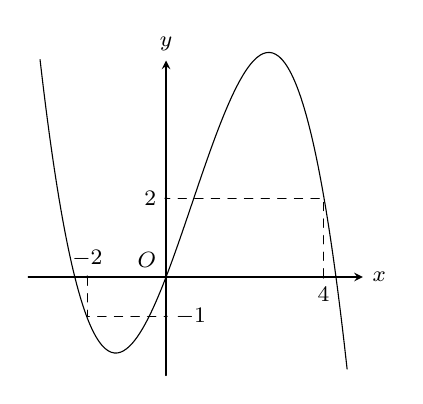
\begin{tikzpicture}[>=stealth,line join=round,line cap=round,font=\footnotesize,scale=0.5]
			\draw[->] (-3.5,0)--(5,0) node[right] {$x$};
			\draw[->] (0,-2.5)--(0,5.5) node[above] {$y$};
			\draw [smooth,domain=-3.2:4.6,samples=100]plot(\x,{-0.26*(\x)^3+0.52*(\x)^2+2.6*(\x)});
			\draw[dashed](-2,0)--(-2,-1)--(0,-1) (4,0)--(4,2)--(0,2);
			\fill (0,0)node[above left]{\footnotesize{$O$}}circle(1.2pt) (4,0)node[below ]{\footnotesize{$4$}}circle(1.2pt) (-2,0)node[above]{\footnotesize{$-2$}}circle(1.2pt) (0,2)node[left]{\footnotesize{$2$}}circle(1.2pt)  (0,-1)node[right]{\footnotesize{$-1$}}circle(1.2pt);
	\end{tikzpicture}}
	\loigiai{\immini{Xét $h(x)=f(x)-\dfrac{x^2}{4}+1$, ta có $h'(x)=f'(x)-\dfrac{x}{2}$.\\
			Dựa vào đồ thị ta có 
			$$h'(x)>0\Leftrightarrow f'(x)>\dfrac{x}{2}\Leftrightarrow\hoac{&x<-2\\&0<x<4.}$$
			Vậy ta có bảng biến thiên của $h(x)$ như hình vẽ.}
		{
			\begin{tikzpicture}[>=stealth,line join=round,line cap=round,font=\footnotesize,scale=0.45]
				\draw[->] (-3.5,0)--(5,0) node[right] {$x$};
				\draw[->] (0,-2.5)--(0,5.5) node[above] {$y$};
				\draw [smooth,domain=-3.2:4.6,samples=100]plot(\x,{-0.26*(\x)^3+0.52*(\x)^2+2.6*(\x)});
				\draw [smooth,domain=-3.5:5,samples=100]plot(\x,{(\x)/2})node[right]{$y=\dfrac{x}{2}$};
				\draw[dashed](-2,0)--(-2,-1)--(0,-1) (4,0)--(4,2)--(0,2);
				\fill (0,0)node[above left]{\footnotesize{$O$}}circle(1.2pt) (4,0)node[below ]{\footnotesize{$4$}}circle(1.2pt) (-2,0)node[above]{\footnotesize{$-2$}}circle(1.2pt) (0,2)node[left]{\footnotesize{$2$}}circle(1.2pt)  (0,-1)node[right]{\footnotesize{$-1$}}circle(1.2pt);
		\end{tikzpicture}}
		\begin{center}
			
\begin{tikzpicture}[scale=1, font=\footnotesize, line join=round, line cap=round, >=stealth]
				\tkzTabInit[nocadre=false, lgt=1.2, espcl=1.8, deltacl=0.6]
				{$x$/0.7, $h'(x)$/0.7,$h(x)$/2.2}
				{$-\infty$,$-2$,$0$,$4$,$+\infty$}
				\tkzTabLine{,+,0,-,0,+,0,-,}
				\tkzTabVar{-/$-\infty$,+/$h(-2)$,-/$h(0)$,+/$h(4)$,-/$-\infty$}
			\end{tikzpicture}
		\end{center}
		Ta có $h(4)=f(4)-4+1=-3$ và $\displaystyle\int\limits_{-2}^4h'(x)\mathrm{\,d}x>0\Rightarrow h(4)>h(-2)$.\\
		Dựa vào bảng biến thiên ta suy ra $h(x)$ có $3$ điểm cực trị và không có giao điểm với trục $Ox$, suy ra hàm số $g(x)=|h(x)|$ có bảng biến thiên như hình vẽ.
		\begin{center}
			
\begin{tikzpicture}[scale=1, font=\footnotesize, line join=round, line cap=round, >=stealth]
				\tkzTabInit[nocadre=false, lgt=2.3, espcl=1.8, deltacl=0.6]
				{$x$/0.7,$h(x)$/2.2,$g(x)=|h(x)|$/2.2}
				{$-\infty$,$-2$,$0$,$4$,$+\infty$}
				\tkzTabVar{-/$-\infty$,+/$h(-2)$,-/$h(0)$,+/$h(4)$,-/$-\infty$}
				\tkzTabVar{+/$+\infty$,-/$|h(-2)|$,+/$|h(0)|$,-/$|h(4)|$,+/$+\infty$}
			\end{tikzpicture}
		\end{center}
		Vậy $g(x)$ có $3$ điểm cực trị, bao gồm $2$ điểm cực tiểu và $1$ điểm cực đại.}
\end{ex}
\begin{ex}%[Thi Chuyên Đề Lần 4 lớp 12 - THPT Trần Phú - Vĩnh Phúc - 23]%[Phan Anh - EX6-2023]%[2D2G6-5]
	Tìm số nghiệm nguyên của bất phương trình $2021^{2x^2-4x+9}-2021^{x^2+5x+1}-(x-1)(8-x)<0$.
	\choice
	{$7$}
	{$5$}
	{\True $6$}
	{$8$}
	\loigiai{Biến đổi bất phương trình ta được
		\begin{eqnarray*}
			&&2021^{2x^2-4x+9}-2021^{x^2+5x+1}-(x-1)(8-x)<0\\
			&\Leftrightarrow&2021^{2x^2-4x+9}-2021^{x^2+5x+1}+x^2-9x+8<0\\
			&\Leftrightarrow&2021^{2x^2-4x+9}+2x^2-4x+9<2021^{x^2+5x+1}+x^2+5x+1.
		\end{eqnarray*}
		Xét $f(t)=2021^t+t$, có $f'(t)=2021^t\ln 2021+1>0$, $\forall t\in\mathbb{R}$ nên $f(t)$ đồng biến trên $\mathbb{R}$.\\
		Bất phương trình đề bài có dạng
		$$f\left(2x^2-4x+9\right)<f\left(x^2+5x+1\right)\Leftrightarrow2x^2-4x+9<x^2+5x+1\Leftrightarrow1<x<8.$$
		Vậy bất phương trình có $6$ nghiệm nguyên.}
\end{ex}
\begin{ex}%[Thi Chuyên Đề Lần 4 lớp 12 - THPT Trần Phú - Vĩnh Phúc - 23]%[Phan Anh - EX6-2023]%[2D2G6-5]
	Có bao nhiêu số nguyên $y$ sao cho ứng với mỗi $y$ có đúng $5$ số nguyên $x$ thỏa mãn $\log\left(x^2+2x+y\right)-2\log(2x-1)>0$
	\choice
	{$75$}
	{$26$}
	{\True $27$}
	{$74$}
	\loigiai{Điều kiện: $\heva{&x^2+2x+y>0\\&2x-1>0}\Leftrightarrow\heva{&x^2+2x+y>0\\&x>\dfrac{1}{2}}$. Biến đổi giả thiết ta được
		$$\log\left(x^2+2x+y\right)-2\log(2x-1)>0\Leftrightarrow x^2+2x+y>(2x-1)^2\Leftrightarrow y>3x^2-6x+1.$$
		Xét $f(x)=3x^2-6x+1$, ta có bảng biến thiên của $f(x)$ như hình vẽ bên dưới
		\begin{center}
			
\begin{tikzpicture}[scale=1, font=\footnotesize, line join=round, line cap=round, >=stealth]
				\tkzTabInit[nocadre=false, lgt=1.2, espcl=4, deltacl=0.6]
				{$x$/1, $f(x)$/2.8}
				{$\dfrac{1}{2}$,$1$,$+\infty$}
				\tkzTabVar{+/$-\dfrac{5}{4}$,-/$-2$,+/$+\infty$}
				\tkzTabVal[draw]{2}{3}{0.3}{$5$}{$46$}
				\tkzTabVal[draw]{2}{3}{0.5}{$6$}{$73$}
			\end{tikzpicture}
		\end{center}
		Để ứng với mỗi $y$, ta có đúng $5$ số nguyên $x$ thỏa bài toán thì $f(5)<y\le f(6)\Leftrightarrow46<y\le73$.\\
		Vậy có $27$ giá trị nguyên của $y$ thỏa yêu cầu bài toán.}
\end{ex}
\begin{ex}%[Thi Chuyên Đề Lần 4 lớp 12 - THPT Trần Phú - Vĩnh Phúc - 23]%[Phan Anh - EX6-2023]%[2H3G3-7]
	Trong KG $Oxyz$ cho mặt phẳng $(P)\colon x-2y+2z+12=0$ và mặt cầu $(S)\colon x^2+y^2+z^2+2x-4y-2z+5=0$. Xét hai điểm $M$, $N$ lần lượt thuộc $(P)$ và $(S)$ sao cho $\overrightarrow{MN}$ cùng phương với véc-tơ $\overrightarrow{u}=(1;1;1)$. Giá trị nhỏ nhất của $MN$ bằng
	\choice
	{$3$}
	{$9\sqrt{3}-1$}
	{\True $6\sqrt{3}$}
	{$2$}
	\loigiai{Mặt phẳng $(P)$ có véc-tơ pháp tuyến là $\overrightarrow{n}=(1;-2;2)$.\\
		Mặt cầu $(S)$ có tâm $I(-1;2;1)$ và bán kính $R=\sqrt{1+4+1-5}=1$.\\
		Ta có $\mathrm{d}(I,(P))=\dfrac{|-1-4+2+12|}{\sqrt{1+4+4}}=3>R$ nên mặt phẳng $(P)$ không có điểm chung với $(S)$.
		\begin{center}
			\begin{tikzpicture}[>=stealth,line join=round,line cap=round,font=\footnotesize,scale=0.7]
				\def\x{-130}
				\path (-1,0.5) coordinate (a)
				(0.2,2) coordinate (b)
				(6,0.5) coordinate (c)
				(3,4) coordinate (I)
				($(I)+({cos(\x)},{sin(\x)})$) coordinate (N)
				($(N)-(0,2)$) coordinate (H)
				($(H)-(1,0)$) coordinate (M)
				($(I)-(0,1)$) coordinate (k)
				($(I)-(0,2.5)$) coordinate (K)
				($(K)+(1,0)$) coordinate (l)
				;
				\draw (I)circle(1);
				\draw (b)--(a)--(c) (N)--(H)--(M)--(N) (k)--(K);
				\draw[dashed](I)--(k);
				\pic[draw,angle radius=2mm,angle eccentricity=1.5] {right angle = I--K--l};
				\foreach \p / \r in {M/-135,H/-45,N/90,I/90}
				\fill (\p) circle (1.2pt) node[shift={(\r:2mm)}]{$\p$};
			\end{tikzpicture}
		\end{center}
		Gọi $\alpha$ là góc tạo bởi $MN$ với mặt phẳng $(P)$. Ta có $\sin\alpha=\dfrac{\left|\overrightarrow{u}\cdot\overrightarrow{n}\right|}{\left|\overrightarrow{u}\right|\cdot\left|\overrightarrow{n}\right|}=\dfrac{|1-2+2|}{\sqrt{1+4+4}\cdot\sqrt{1+1+1}}=\dfrac{1}{3\sqrt{3}}$.\\
		Gọi $H$ là hình chiếu của $N$ lên $(P)$. Ta có
		$$MN=\dfrac{NH}{\sin\alpha}=3\sqrt{3}NH\ge3\sqrt{3}\left(\mathrm{d}(I,(P))-R\right)=3\sqrt{3}(3-1)=6\sqrt{3}.$$
		Vậy giá trị nhỏ nhất của $MN$ bằng $6\sqrt{3}$.}
\end{ex}

\Closesolutionfile{ans}
\begin{indapan}{10}
	{ans/ans-2-TT-21-TranPhu-VinhPhuc-L4-23}
\end{indapan}


